%%%%%%%%%%%%%%%%%%%%%%%%%%%%%%%%%%%%%%%%%%%%%%%%%%%%%%%%%%%%%%%%%%%%%%
\section{Architecture technique}
%%%%%%%%%%%%%%%%%%%%%%%%%%%%%%%%%%%%%%%%%%%%%%%%%%%%%%%%%%%%%%%%%%%%%%

L'architecture proposée est volontairement modulaire : la collecte, les
métadonnées, le stockage audio et le pipeline de préparation sont
séparés, ce qui facilite la maintenance et l'ajout futur de modules de
traitement automatique de la parole.

\begin{figure}[H]
\centering
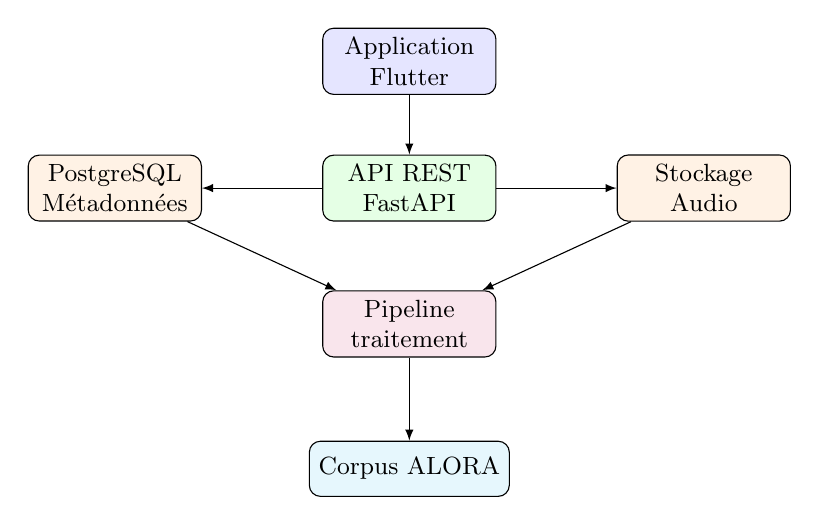
\begin{tikzpicture}[x=1.7cm,y=1.15cm,
 every node/.style={draw,rounded corners,minimum width=2.2cm,minimum height=0.7cm,align=center,font=\small},
 >=latex
]

\node[fill=blue!10] (client) at (0,3) {Application\\Flutter};
\node[fill=green!10] (api) at (0,1.6) {API REST\\FastAPI};
\node[fill=orange!10] (db) at (-2.2,1.6) {PostgreSQL\\Métadonnées};
\node[fill=orange!10] (storage) at (2.2,1.6) {Stockage\\Audio};
\node[fill=purple!10] (pipeline) at (0,0.1) {Pipeline\\traitement};
\node[fill=cyan!10] (dataset) at (0,-1.5) {Corpus ALORA};

\draw[->] (client)--(api);
\draw[->] (api)--(db);
\draw[->] (api)--(storage);
\draw[->] (db)--(pipeline);
\draw[->] (storage)--(pipeline);
\draw[->] (pipeline)--(dataset);

\end{tikzpicture}
\caption{Vue d'ensemble de l'architecture proposée}
\end{figure}

\begin{table}[H]
\centering
\begin{tabular}{p{3.2cm}p{9cm}}
\toprule
\textbf{Composant} & \textbf{Rôle} \\
\midrule
Flutter & Application mobile/web de collecte et de validation des enregistrements. \\
FastAPI & Backend de gestion des utilisateurs, des fichiers audio et des métadonnées. \\
PostgreSQL & Stockage des données structurées : locuteurs, sessions, prompts et annotations. \\
Stockage audio & Conservation des fichiers bruts et validés, séparés des métadonnées. \\
Pipeline & Validation, transcription, segmentation, annotation et export du corpus. \\
\bottomrule
\end{tabular}
\caption{Composants clés de la première phase}
\end{table}

Ce découpage permet de faire évoluer la collecte et le traitement de
façon indépendante, tout en conservant une base commune de données
exploitables pour les futurs modèles d'apprentissage automatique.